\indent Para corroborar el correcto funcionamiento de nuestro algoritmo implementado desarrollamos los siguientes tests:\\


\begin{center}
 \textbf{Sin Soluci\'on}
\end{center}

Este caso se da cuando el nodo que representa a la estaci\'on final queda aislado  \\

El grafo que representa a este tipo es de la siguiente forma:\\

\vspace*{0.3cm} \vspace*{0.3cm}
  \begin{center}
 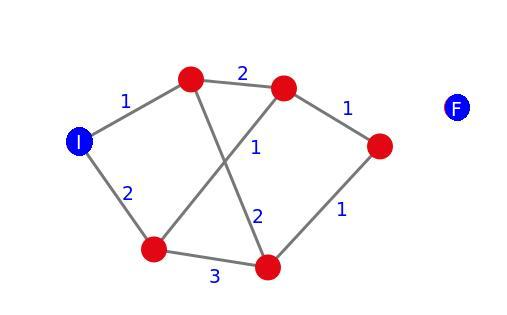
\includegraphics[scale=0.5]{./EJ3/grafoSinSolucion.jpeg}
 \\{$Ejemplo$ \ 3.1 - $Caso$ $Sin$ $Soluci$\'on}
  \end{center}
  \vspace*{0.3cm}
  
\begin{center}
 \textbf{Sin ejes}
\end{center}

Esta familia de casos se da cuando todos los nodos que representa a la estaciones quedan aislados  \\

El grafo que visualiza a este tipo presenta la siguiente forma:\\

\vspace*{0.3cm} \vspace*{0.3cm}
  \begin{center}
 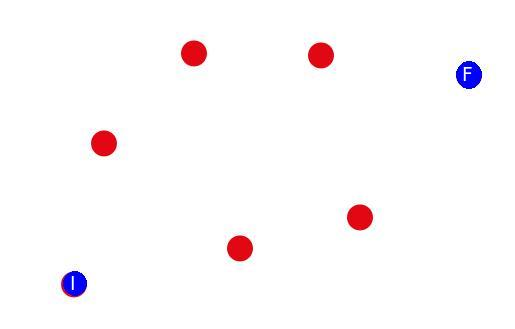
\includegraphics[scale=0.5]{./EJ3/grafoSinEjes.jpeg}
 \\{$Ejemplo$ \ 3.2 - $Caso$ $Sin$ $Ejes$}
  \end{center}
  \vspace*{0.3cm}

\begin{center}
 \textbf{Camino simple}
\end{center}

Este caso se da cuando el grafo que se recibe como par\'ametro ya presenta un camino simple armado desde la estaci\'on inicial a la final

El grafo que describe a esta familia de casos es el siguiente:\\

\vspace*{0.3cm} \vspace*{0.3cm}
  \begin{center}
 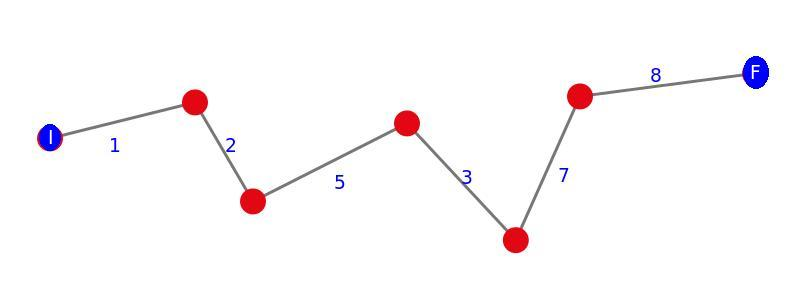
\includegraphics[scale=0.5]{./EJ3/grafoCaminoSimple.jpeg}
 \\{$Ejemplo$ \ 3.3 - $Caso$ $Camino$ $Simple$}
  \end{center}
  \vspace*{0.3cm}
  
\begin{center}
 \textbf{Multiples caminos de igual peso llegan a destino}
\end{center}

Este caso se da cuando existen varios ramas dentro del grafo que van desde el nodo inicial hasta el \'ultimo y la suma de dichos pesos termina siendo igual. Veremos m\'as adelante que por la implementaci\'on y desarrollo de nuestro algoritmo este terminar\'a siendo el peor caso.


El grafo que describe a esta familia de casos es el siguiente:\\

\vspace*{0.3cm} \vspace*{0.3cm}
  \begin{center}
 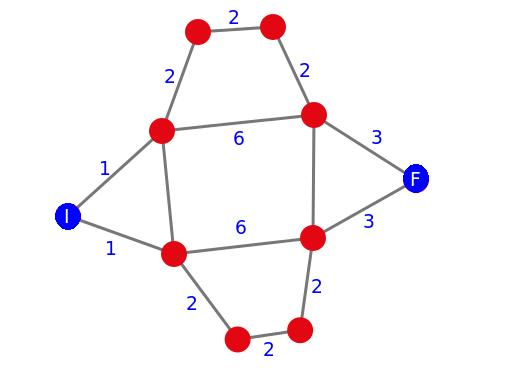
\includegraphics[scale=0.5]{./EJ3/grafoMultiCamino.jpeg}
 \\{$Ejemplo$ \ 3.4 - $Caso$ $Con$ $Multiples$ $Caminos$}
  \end{center}
  \vspace*{0.3cm}
  
\begin{center}
 \textbf{Caso random}
\end{center}

Este caso se da cuando se recibe grafos con aristas y nodos sin ninguna particularidad.

